%!TEX root = ../physical-olympics-2.tex
\chapter{磁生电}

\section{电磁感应}

静止电荷产生的静电场, 稳恒电流产生的静磁场, 这些都已经被我们研究地足够充分了. 是时候, 我们也该思考以下问题:
\begin{enumerate}
\item 如果电荷不是完全静止, 静电场是否会有改变?
\item 如果电荷不是完全静止, 会不会产生一个磁场?
\item 如果电流不是完全稳恒, 静磁场是否会有改变?
\item 如果电流不是完全稳恒, 会不会产生一个电场?
\end{enumerate}

其中问题$1,\,3$在我们看来已经有答案: 非静止的, 非稳恒的源自然要产生非静电场和非静磁场, 至少产生的场需要相对元产生一定的推迟. 问题$2,\,4$就值得更进一步地研究. 其中问题$2$的答案是可以被推理出来的, 它就是下一章麦克斯韦发现的重要现象: 不能单独假设只有电流会产生磁场, 不然磁场的旋度将不会自洽, 从而根据电荷守恒发现只需要假设电荷运动造成的变化的电场也能造成一个磁场. 尽管第三点更容易被解释. 但是历史地看, 人们更早地得到了问题$4$的答案: 变化的磁场(源于非稳恒的电流)必然造成一个新的电场, 它完全独立于电荷产生的那一类电场, 因为这个电场有旋度而无散度. 它被称作\emph{涡旋电场}(eddy electric field).

在对历史上的背景做一个回顾前重新探讨一下此前概念的定义是有必要的. 我们有洛伦兹力公式:
\[\bs{F}=q(\bs{E}+\bs{v}\times\bs{B})\]

这个表达式实际上构成了描述电场, 磁场强度的量$\bs{E},\,\bs{B}$的唯一操作性定义: 只需要在空间中放置试探电荷$q$, 并给它一个测试速度$\bs{v}$就可以通过受力的结果定义空间该点的电磁场. 它的普遍性与协变性只能通过实验来验证, 两者都是随时间变化的矢量场, 且其值依赖于参考系的选取:
\[\bs{E}=\bs{E}(\bs{r},\,t)\quad,\quad \bs{B}=\bs{B}(\bs{r},\,t)\]
\[(\bs{E},\,\bs{B})\overset{\bs{v}}{\longrightarrow}(\bs{E}',\,\bs{B}')\]

而暂时取消关于电势与矢势的定义. 很难想像如何在电场可能有旋, 磁场可能有散的情形下依然承认:
\[\bs{E}=-\nabla\varphi\]
\[\bs{B}=\nabla\times\bs{A}\]

因为我们记得梯度一定无旋, 旋度一定无散:
\[\nabla\times\nabla\varphi=0\quad ,\quad \nabla\cdot\nabla\times\bs{A}=\bs{0}\]


于是现在问题变成了, 要研究通过此前式子定义的二分量电磁场$(\bs{E},\,\bs{B})$是如何依赖于产生它们的电荷的运动形式的(注意, 后面还讲证明存在不由电荷产生的电磁场). 历史背景上最早被发现的性质莫过于\emph{法拉第电磁感应定律}(Faraday's law of induction), 它的一个现代版本的表述为:
\[\oint\limits_{\partial V}\left(E_x\ud t\ud x+E_y\ud t\ud y+E_z\ud t\ud z+B_x\ud y\ud z+B_y\ud z\ud x+B_z\ud x\ud y\right)=0\]

\begin{wrapfigure}[13]{o}[-10pt]{8cm}
\vspace{-0.4cm}
\centering
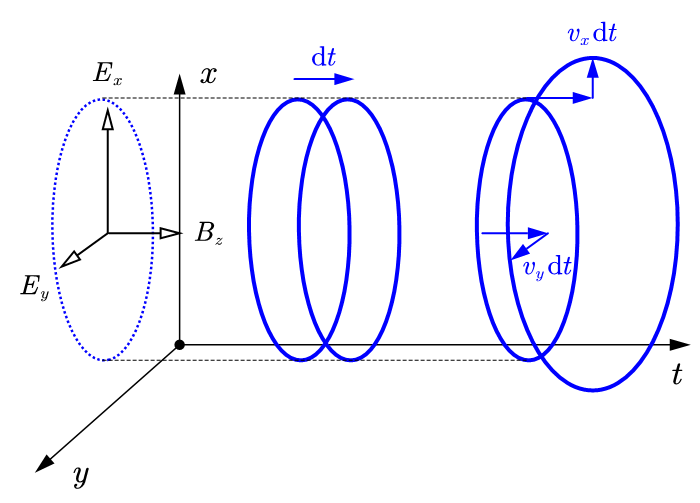
\includegraphics[width=8cm]{image/7-5-1.png}
\caption{法拉第电磁感应定律}\label{fig:7-5-1}
\end{wrapfigure}
其中$\partial V$表示任意一个四维时空中一个三维体的边界. 而如果取这个体为一个三维空间中静止的二维曲面以一个非常短的时间间隔$\ud t$为高形成的柱体造成的边界, 上式就变成了我们可能更熟悉的式子:
\[\left(\oint\limits_{\partial \bs{A}}\bs{E}\cdot\ud\bs{l}\right)\ud t+\int\limits_{t+\ud t,\,\bs{A}}\bs{B}\cdot \ud\bs{A}-\int\limits_{t,\,\bs{A}}\bs{B}\cdot \ud\bs{A}=0\]
\[\Rightarrow \quad \oint\limits_{\partial \bs{A}}\bs{E}\cdot\ud\bs{l}=- \frac{\ud\Phi_{\bs{A}}}{\ud t}\]

这个式子被当时的诸多物理学家(法拉第, 亨利, 楞次等)在实验室里测量验证. 它无可辩驳地证明了在变化的电磁场下, 电场将会成为有旋的场, 过去理论的根基无疑发生了动摇.

十分有意思的是, 另一个相关的结果也同时被研究了: 当我们考虑的不是一个四维空间的母线沿时间方向的柱体, 而是如图\ref{fig:7-5-1}那样上底下底不一样(但依然垂直于时间轴)的台状体, 实际上就是一个在运动的线圈(不限于平移, 可以扩大缩小或任意弯曲). 设线圈边缘的速度为$\bs{v}$, 那么在侧面也会造成一个磁场积分的分量, 上式就会变成:
\[\Rightarrow \quad \oint\limits_{\partial \bs{A}}\bs{E}\cdot\ud\bs{l}=- \frac{\ud\Phi_{\bs{A}}}{\ud t}-\oint\limits_{\partial \bs{A}}(\bs{v}\times\bs{B})\cdot\ud\bs{l}\]

\[\Rightarrow \quad \oint\limits_{\partial \bs{A}}(\bs{E}+\bs{v}\times\bs{B})\cdot\ud\bs{l}=- \frac{\ud\Phi_{\bs{A}}}{\ud t}\]

上式左侧恰好又变成了完整的洛仑兹力(单位电荷受到的). 事实上在实验室它也只能作为一个整体被测量, 上式左侧其实就是实验室测得的线圈上的电动势, 两项分别构成了感生电动势与动生电动势, 右侧则是线圈包含的磁通量对时间的导数. 从而一个更复杂但也更浅显易懂的法拉第电磁感应定律表述为:
\[\mathscr{E}=\oint\bs{K}\cdot \ud \bs{l}=-\frac{\ud\Phi}{\ud t}\]
\[\mathscr{E}=\mathscr{E}_{\rm transformer}+\mathscr{E}_{\rm motional}\]
\[\mathscr{E}_{\rm motional}=\oint\bs{E}\cdot\ud\bs{l}\]
\[\mathscr{E}_{\rm transformer}=\oint(\bs{v}\times\bs{B})\cdot\ud\bs{l}\]

但是, 法拉第电磁感应定律又不全然是实验定律, 背后体现的相对论协变性是不难理解的. 我们从本章的论述就会逐渐明白这一点.


\subsection{动生电动势}

\emph{动生电动势}(motional electromotive force)并不是什么新奇的现象. 在静磁场下我们足以理解动生电动势, 它只不过是上一章就研究过的磁场力的另一个效应, 此时存在非静电力:
\[\bs{K}=\bs{v}\times \bs{B}\]

考虑它沿导线方向的分量对回路积分就是此前在稳恒电流章节中介绍的电动势:
\[\mathscr{E}=\oint(\bs{v}\times\bs{B})\cdot\ud\bs{l}\]

上式经常会被被表述为: 导线单位时间切割的磁感线根数. 这样的表述的合理性在于, 注意到上式中的三重标积可以化为:
\[(\bs{v}\times\bs{B})\cdot\ud\bs{l}=\bs{B}\cdot(\ud\bs{l}\times\bs{v}) \]

点乘后就是导线元扫过的面元, 故积分的项的确也就表示扫过的面积上的磁通量, 从而不难理解这类电动势自动就符合法拉第电磁感应定律:
\[\mathscr{E}=-\frac{\ud\Phi}{\ud t}\]

如果考虑导线中的电荷沿导线方向的另一个速度造成的电流$I$, 那么其电流元就会导致一个安培力:
\[\ud\bs{F}=I\ud\bs{l}\times \bs{B}\]

一段电路动生电动势做功的功率:
\[\ud P_{\mathscr{E}}=\ud \mathscr{E}\cdot I=I(\bs{v}\times \bs{B})\cdot \ud\bs{l}\]

该功率变成了电路内部的能量. 是注意到安培力作为磁场力的另外一个分力也要做功, 功率为:
\[\ud P_A=\ud \bs{F}\cdot \bs{v}=I(\ud\bs{l}\times \bs{B})\cdot  \bs{v}\]

这个功将转化为导线的机械能. 那么由于磁场力本质上不会做功, 这一点很容易就能够利用三重标积公式在两个功率上得到印证:
\[\ud P_{\mathscr{E}}+\ud P_A=0\]

从而两个功率的大小代表机械能和电能转化的快慢.\,对于电动机,\,电能转化为机械能,\,对于发电机,\,机械能转化为电能.

事实上即使对于变化的电磁场, 其中磁场也是永远不做功的. 这一点从磁场的操作定义式就可以看出来, 磁场力作为速度与磁场的叉乘是垂直于速度的. 但要注意, 一般\emph{不说洛伦兹力不做功}, 因为电场力也要算作是洛伦兹力的一部分, 洛伦兹力没有道理不包括电场力.

当动生电磁感应发生在一个变化的电磁场中运动的线圈上时, 根据$\bs{v}\times \bs{B}$在线圈上的积分给出了整个感应电动势贡献中的一项, 实际磁通量的导数才对应总的感应电动势, 而动生电动势相当于把磁场视作常数求导得到的值:
\[\mathscr{E}_{\rm motional}=-\left.\frac{\ud \Phi}{\ud t}\right|_{B\text{不变}}\]

\subsection{感生电动势}

动生电动势并没有带来新的物理现象. 但是它的结果却给我们以启示: 磁通量的改变与导线中的感应电动势有关. 那么只需要稍微思考一下另外的参考系中观察者看到的现象就不难推理出另一种感应电动势的可能.

相对性原理容易说明, 如果产生磁场的物质在发生运动以致使其发生变化, 那么即使线圈静止,\,也会产生感应电动势. 那么内部电荷受到的非静电力就必然不是磁场力, 因为根据电磁场的定义:
\[\bs{F}=q(\bs{E}+\bs{v}\times\bs{B})\]

而现在线圈$\bs{v}=\bs{0}$. 我们只能把这个力称作电场力. 这种电场称作\emph{感生电场}(induced electric field). 有时, 它被理解为变化的磁场产生的, 这其实是因为在线圈看来电动势公式应该\footnote{在忽略某些可能的相对论效应的意义下.}是:
\[\oint\limits_{\partial \bs{A}}\bs{E}\cdot\ud\bs{l}=-\frac{\ud\Phi}{\ud t}=-\int\limits_{\bs{A}} \frac{\partial \bs{B}}{\partial t}\cdot\ud\bs{A}\]

这个式子的直接推论就是:
\[\nabla\times\bs{E}=- \frac{\partial \bs{B}}{\partial t}\]

这个式子与电流产生磁场的数学结构相似性:
\[\nabla\times \bs{B}=\mu_0\bs{j}\]


暗示了把磁场的改变看作电场的一类源似乎是合适的, 的确从操作性上可以这么做, 甚至原来静磁学中的一切电流产生磁场的结论都可以原封不动地用来求变化的磁场下的感生电场. 但事实上, 我们还有两个更加本质的看法.

一是把感生电场看作静磁场的相对论效应, 这又和上一章静磁场开头时把磁场本身看作电场的相对论效应的做法如出一辙. 原参考系中的速度为$v_x,\,v_y,\,v_z$, 而具有磁场$B_x,\,B_y,\,B_z$时受力为:
\[F_x=q(v_yB_z-v_zB_y)\]
\[F_y=q(v_zB_x-v_xB_z)\]
\[F_z=q(v_xB_y-v_yB_x)\]

这一次倒好, 我们连近似都不做了, 直接认为一个相对原系以$u$沿$x$方向运动的参考系下受力就是原系中的受力:
\[F_x'=F_x\quad ,\quad F_y'=F_y\quad ,\quad F_z'=F_z\]

用经典的速度叠加:
\[v_x=v_x'+u\quad ,\quad v_y=v_y' \quad ,\quad v_z=v_z'\]

得到:
\[F_x'=q(v_y'B_z-v_z'B_y)\]
\[F_y'=-quB_z+q(v_z'B_x-v_x'B_z)\]
\[F_z'=quB_y+q(v_x'B_y-v_y'B_x)\]

从而由洛伦兹力公式, 的确在新参考系中产生了电场:
\[E_x'=0\quad ,\quad E_y'=-uB_z\quad ,\quad E_z'=uB_y\]

这实际上就是:
\[\bs{E}=\bs{u}\times\bs{B}\]

故如果一个点相对一个稳恒电流体系以$-\bs{v}$运动, 即稳恒电流体系相对这个点具有均匀的速度$\bs{v}$时, 这个点产生的涡旋电场就是:
\[\bs{E}=-\bs{v}\times\left(\int \kb\frac{\bs{j}\times \bs{e}_{\bs{R}}}{R^2}\ud V\right)\]

而如果电流的各个部分不一致, 由叠加原理也可以得到表达式:
\[\bs{E}=\int \kb\frac{(\bs{j}\times \bs{e}_{\bs{R}})\times\bs{v}}{R^2}\ud V\]

我们不加证明地指出上式可以通过矢量微分的方法化简成我们马上要得到的形式, 这就是第二种涡旋电场产生的条件的理解方式: 变化的磁场事实上又由变化的电流产生. 最终连接感生电场与其源头: 变化的电流的, 是以下公式:
\[\bs{E}=-\frac{\partial \bs{A}}{\partial t}=-\int \frac{\mu_0}{4\pi}\frac{\frac{\partial \bs{j}}{\partial t}}{r^2}\ud V\]

请注意, 我们又非常奇妙地定义了一个磁矢势. 这是因为我们依然将磁场体系视作\emph{准恒}(quasistatic)的. 即磁场主导的情况下, 磁场场源运动速度远小于光速以至于产生的电场$E\ll cB$. 从而磁矢势就被``近似''定义为与静磁场一样的电流的体积分:
\[\bs{A}=\int \frac{\mu_0}{4\pi}\frac{\bs{j}}{r^2}\ud V\]

 唯一要注意的是, 由于$\nabla\cdot\bs{A}=0$依赖于电流的稳恒性条件, 以至于它和$\nabla^2\bs{A}=-\mu_0\bs{j}$都从原理上不再准确. 将上式对回路进行积分便得到同样的感生电动势公式作为其正确性的一个验证:
\[\mathscr{E}=\oint \bs{E}\cdot\ud \bs{l}=-\frac{\partial }{\partial t}\oint \bs{A}\cdot \ud \bs{l}=-\frac{\ud \Phi}{\ud t}\]

我们趁热也来看看准恒情况下关于电场电势的定义. 诚然我们不能为真实的电场定义一个电势$\varphi$使它满足:
\[-\nabla\varphi=\bs{E}\]

因为此时的电场是涡旋的. 但是仿照之前磁矢势的``近似''定义, 我们自然也可以自然地``近似''定义电标势为:
\[\varphi=\int \ke\frac{\rho}{r^2}\ud V\]

那么, 留下的一个矛盾就变成了:
\[\bs{E}\neq -\nabla\varphi\]

这也没啥古怪的, 实际上在准恒条件下``近似''成立\footnote{例如让体系以小量角频率$\omega$发生振动, 那么下式在$\omega$一阶下精确.}的一个式子为:
\[\bs{E}=-\nabla\varphi-\frac{\partial \bs{A}}{\partial t}\]

这样就把电场分为了两个部分, 一个是只与每时每刻的净电荷分布有关的``静电场''分量, 一个是由电流的改变造成的``涡旋电场''分量. 而电势总是定义在前者上的. 

事实上我们此前稳恒电流章节大量使用到了电路中各点的电势, 在涡旋电场遍布电路中的各个支路时, 这个电势实际上也就是我们现在所阐明的电势概念. 更特别地, 把$-\frac{\partial \bs{A}}{\partial t}$视作非静电力$\bs{K}$, 而如果电路中电荷除了受到静电力$-\nabla\varphi$和非静电力$\bs{K}$外不受其他非静电力, 即有微观欧姆定律$\bs{E}=\rho\bs{j}$, 在准恒或稳恒的条件下对支路进行积分, 就得到了部分电路的欧姆定律:
\[IR=\Delta \varphi+\mathscr{E}\]

如果将上式乘以电流, 就得到能量等式:
\[I^2R=UI+\mathscr{E}I\]

尤其是对回路而言, 电压一圈下来没有改变:
\[I^2R=\mathscr{E}I\]

那么其焦耳热来源为感生电磁感应的电动势对电流的做功$\mathscr{E}I$. 因为是电场所以是可以做功的. 但是其实这个感生涡旋电场本身作为磁场变化的产物而能量远低于磁场能量, 所以其实最终能量来自于磁场里的能量. 下一章我们将讨论电磁场整体的能量. 现在不妨这么想: 涡旋电场对感应线圈上的电流做了功, 那么就必然存在运动的场源电流, 而它们又置身于感应线圈上的电流产生的磁场中, 从而移动它们需要外力做额外的功, 很多情况下正是这个功在补偿从磁场中通过电磁感应漏向电场的能量.


当感生电磁感应发生在一个变化的电磁场中运动的线圈上时, 根据$\bs{E}=-\frac{\partial \bs{A}}{\partial t}$在线圈上的积分给出了整个感应电动势贡献中的一项, 实际磁通量的导数才对应总的感应电动势, 而感生电动势相当于把线圈视作不动求导得到的值:
\[\mathscr{E}_{\rm transformer}=-\left.\frac{\ud \Phi}{\ud t}\right|_{\bs{A}\text{不变}}\]


将感应电动势的动生和感生部分合并,\,得到完整的法拉第电磁感应定律:
\[\mathscr{E}=-\left.\frac{\ud \Phi}{\ud t}\right|_{B\text{不变}}-\left.\frac{\ud \Phi}{\ud t}\right|_{\bs{A}\text{不变}}=-\frac{\ud \Phi}{\ud t}\]


\section{自感与互感}

\begin{itemize}
\item 自感定义与自感系数公式:
\[\Psi=LI\quad ,\quad L=\frac{\mu N^2 S}{l}\]

\item 两线圈互感时的相关公式:
\[E=\frac{1}{2}L_1I_1^2+\frac{1}{2}L_2I_2^2+ MI_1I_2\]

\[\Psi_1=L_1I_1+MI_2\quad \Rightarrow\quad  U_1=-L_1\frac{\ud I_1}{\ud t}-M\frac{\ud I_2}{\ud t}\]
\[\Psi_2=L_2I_2+MI_1\quad \Rightarrow\quad  U_2=-L_2\frac{\ud I_2}{\ud t}-M\frac{\ud I_1}{\ud t}\]
\[U_1I_1+U_2I_2=-\frac{\ud E}{\ud t}\]
\end{itemize}

